\documentclass[10pt,a4paper,catalan]{article}
\usepackage[latin1]{inputenc}
%\usepackage[T1]{fontenc}
\usepackage{babel}
\usepackage[a4paper,left=2cm,right=2cm,top=3cm,bottom=3cm]{geometry}
%\usepackage{amsmath}
%\usepackage{amsfonts}
%\usepackage{amssymb}
\usepackage[pdftex,bookmarks=true,pdfborder={000}]{hyperref}
\usepackage{xcolor}
\usepackage{listings}
%\usepackage{caption}
\usepackage{graphicx}
\usepackage{float}
\usepackage{subfig}


\DeclareCaptionFont{white}{\color{white}}
\DeclareCaptionFormat{listing}{\colorbox{gray}{\parbox{\textwidth}{#1#2#3}}}
\captionsetup[lstlisting]{format=listing,labelfont=white,textfont=white}

\definecolor{gray97}{gray}{.97}
\definecolor{gray75}{gray}{.75}
\definecolor{gray45}{gray}{.45}

\lstset{
  frame=Ltb,
  language=C,
  captionpos=t,
  tabsize=2,
  framerule=0pt,
  framextopmargin=5pt,
  framexbottommargin=3pt,
  framexleftmargin=0.4cm,
  framesep=0pt,
  rulesep=.4pt,
  backgroundcolor=\color{gray97},
  rulesepcolor=\color{black},
  showstringspaces = false,
  keywordstyle=\bfseries\color{blue},
  commentstyle=\color{teal},
  stringstyle=\ttfamily\color{red},
  numbers=left,
  numbersep=15pt,
  numberstyle=\tiny,
  numberfirstline = false,
  breaklines=true,
  showstringspaces=false,
  basicstyle=\ttfamily\footnotesize,
  emph={label}
}

\newcommand{\unit}[1]{\ensuremath{\, \mathrm{#1}}}

%opening
\title{Pr\'actica 4: Utilizaci\'on de controladores de instrumentos. Errores sistem\'aticos}
\author{Dani Gabriel y Rafael G\'omez}
\date{Abril 2011}

\begin{document}

\pagebreak

\maketitle

\tableofcontents

\pagebreak

\section{Estudio Previo}

\begin{figure}[H]
 \centering
 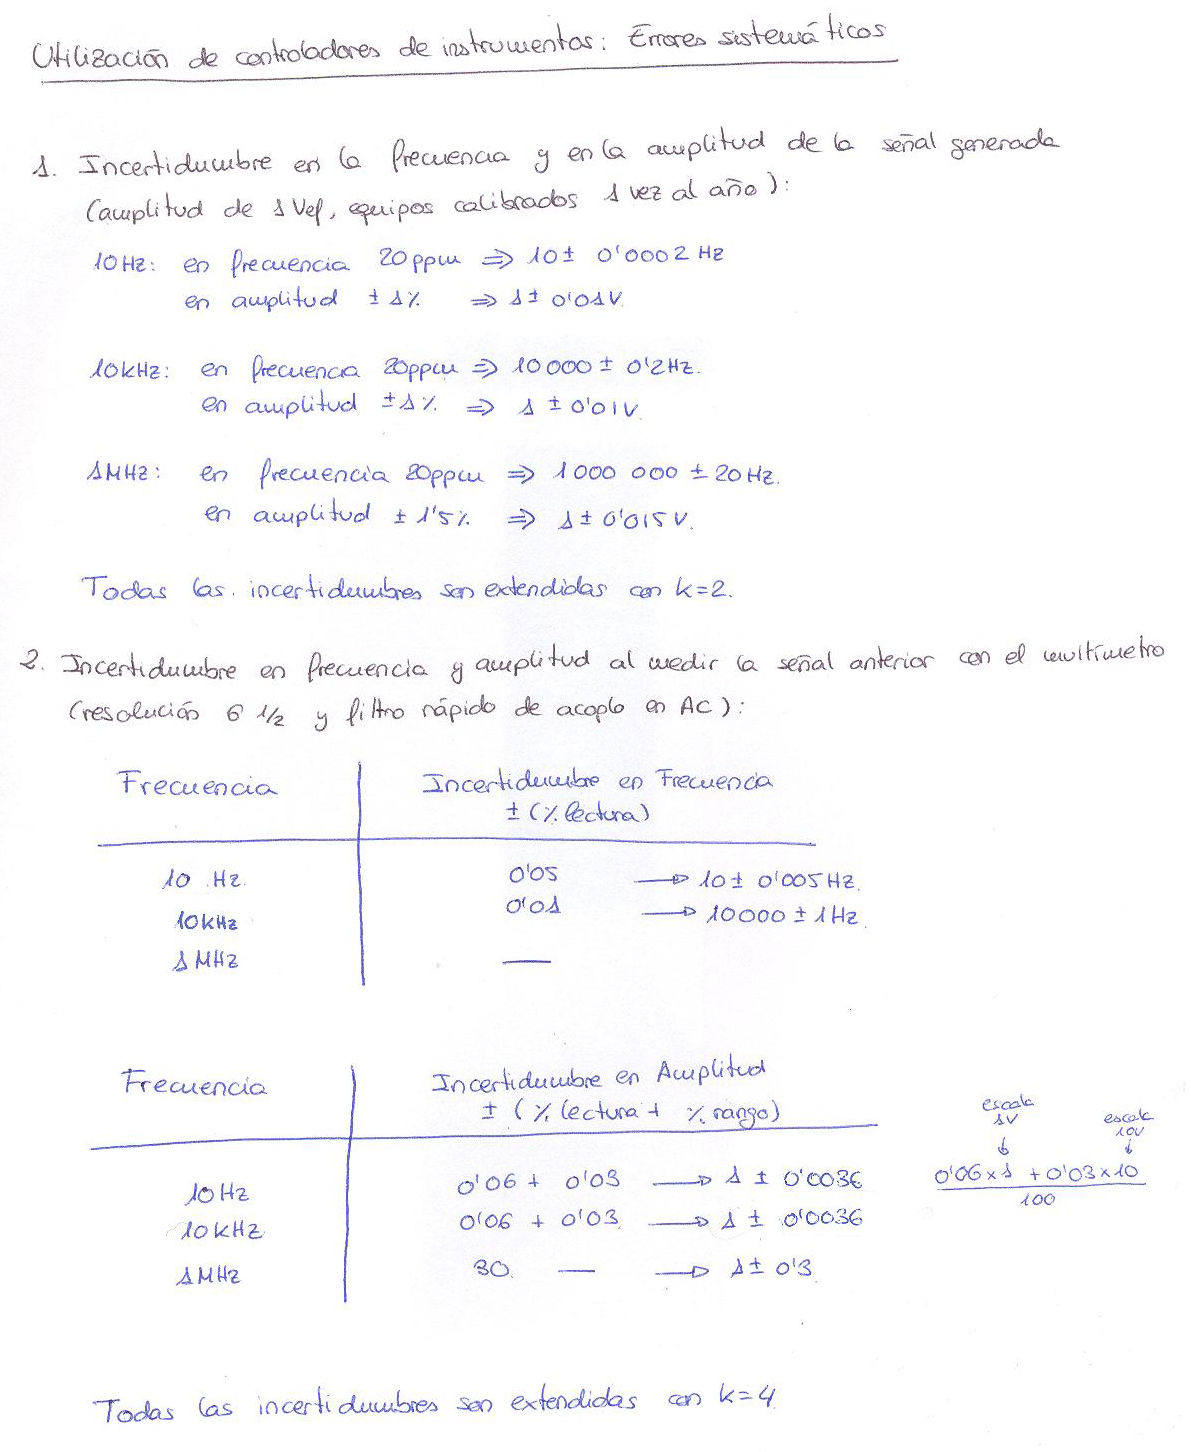
\includegraphics[width=1\textwidth]{previos}
\end{figure} 

\section{Trabajo de Laboratorio}

\subsection{Dise�o del VI}

Se pretende dise�ar un VI que controle el generador de funciones y el mult�metro, de manera que el panel frontal permita modificar la frecuencia, amplitud y forma de onda, y muestre los valores de la frecuencia y amplitud programadas, medidas, y la diferencia entre ellas. Puede verse el instrumento en la figura \ref{fig:ej1}.

\begin{figure}[H]
 \centering
 \subfloat[Panel Frontal]{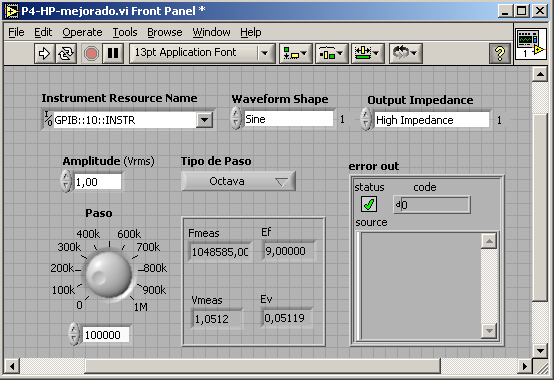
\includegraphics[width=0.6\textwidth]{frontal}}
 \vspace{0.5cm}
  \subfloat[Diagrama de Bloques]{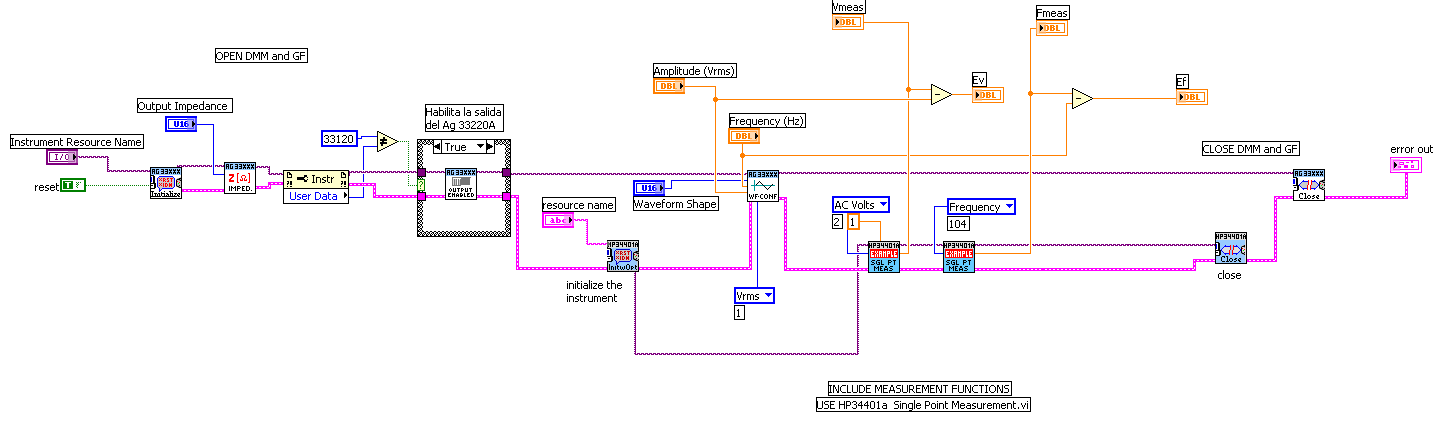
\includegraphics[width=1\textwidth]{bloquesp41}}
 \vspace{0.5cm}
 \caption{Instrumento Dise�ado}
 \label{ej1}
\end{figure}

\subsection{Verificaci�n de medidas y errores}

Realizamos una medida y comprovamos si el resultado obtenido est� dentro de los m�rgenes especificados por el fabricante. Programamos una se�al sinusoidal de $1Vef$ y frecuencia de 10 kHz. Las lecturas que obtenemos son:

\begin{itemize}
 \item $f = 10000,08$
 \item $V = 0,996700$
\end{itemize}

Calculamos el error especificado por el fabricante para el voltaje mediante la ecuaci�n \ref{eq:eq-err} y vemos que efectivamente, el error medido (0,0033) es menor que el especificado. N�tese que no nos dimos cuenta y que el rango lo pusimos a $10V$, que no es lo optimo para medir $1Vef$.

\begin{equation}
 \frac{0,03*escalaLectura+0,06*rango}{100}= 3,6*10^{-3} = \frac{0,03*1+0,06*10}{100}= 3,6*10^{-3} \label{eq:eq-err}
\end{equation}

\vspace{0.5cm}
La frecuencia tambi�n se halla dentro de la incertidumbre especificada por el fabricante (0.2Hz).

\subsection{Verificaci�n de errores sistem�ticos}

Con la misma se�al que en el apartado anterior (senoidal, 1Vef, 10kHz) tomamos varias medidas:\\

\begin{tabular}{|l|l|l|l|}
 \hline
 {\bf Frecuencia medida (Hz)} & {\bf Error de frecuencia (Hz)} & {\bf Tensi�n medida (V)} & {\bf Error de tensi�n (V)} \\
 \hline
 10000.08 & 0.08 & 0.96700 & -0.003300 \\ 
 \hline
 10000.08 & 0.08 & 0.96700 & -0.003350 \\
 \hline
 10000.08 & 0.08 & 0.96700 & -0.003300 \\
 \hline
 10000.08 & 0.08 & 0.96700 & -0.003400 \\
 \hline
 10000.08 & 0.08 & 0.96700 & -0.003500 \\
 \hline
 10000.07 & 0.07 & 0.96600 & -0.003420 \\
 \hline
 10000.08 & 0.08 & 0.96600 & -0.003310 \\
 \hline
 10000.08 & 0.08 & 0.96500 & -0.003460 \\
 \hline
 10000.08 & 0.08 & 0.96400 & -0.003600 \\
 \hline
 10000.08 & 0.08 & 0.96300 & -0.003730 \\
 \hline
\end{tabular} \\  

Despu�s de observar la tabla, podemos establecer que existe un error aleatorio en la frecuencia de $\pm 0.01Hz$ que se produce con una probabilidad muy baja, mientras que en tensi�n, pueden distinguirse frecuentes errores de $\pm 0.000430 V$.

\subsection{Verificaci�n del tipo de conversor AC/DC}

Programamos ahora una se�al cuadrada de 1Vef y 10kHz con el generador de funciones. Con esto pretendemos verificar si el conversor alterna-continua del mult�metro es de Verdadero Valor Eficaz (calcula el valor eficaz de la se�al correctamente, independientemente del tipo de se�al) o no (calcula el valor eficaz de manera correcta solo para se�ales senoidales, ya que siempre aplica al valor de pico el factor $1/\sqrt{2}$)

Tras realizar la medida, el valor de la tensi�n obtenida es 1.00010 V, por lo que podemos observar que se corresponde con el valor eficaz de la tensi�n programado en el generador. As� pues, concluimos en que tenemos un conversor de Verdadero Valor Eficaz.

\subsection{Verificaci�n de medidas extremas}

A continuaci�n comprovaremos los resultados de medir una se�al senoidal de 1Vef a 10Hz y a 1MHz para ver si los resultados obtenidos se ajustan a las especificaciones del fabricante.

Para el caso de 10Hz, la lectura que obtenemos es de 0.7857 V, que se pasa en mucho de la incertidumbre esperada (0.0036 V seg�n el previo)

Para el caso de 1MHZ, la lectura es de 1.03529 V y la incertidumbre, por tanto, es de 0.035 V, que se ajusta dentro del margen establecido por el fabricante a 0.3V para esta frecuencia.


\section{Trabajo Opcional}

\subsection{Implementaci�n de un sistema de barrido de frecuencias}

Utilizando el VI anterior, vamos a crear uno que haga un barrido de frecuencias entre una m�xima y una m�nima con paso seleccionable. Para poder recoger los resultados de cada medida de manera pr�ctica y c�moda, nuestra implementaci�n incluye la escritura de las medidas en un fichero .txt (Ver figura \ref{fig:vimejorado}).

\begin{figure}[H]
 \centering
 \subfloat[Panel Frontal]{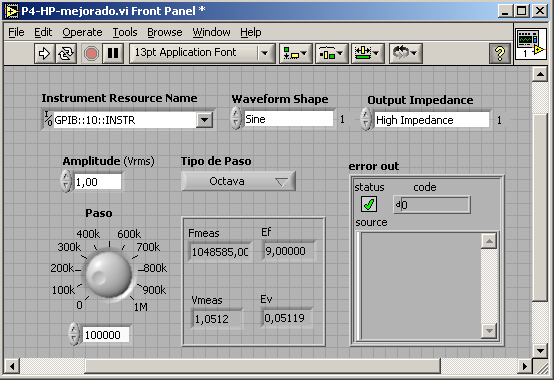
\includegraphics[width=0.6\textwidth]{frontal}}
 \vspace{0.5cm}
 \subfloat[Diagrama de Bloques]{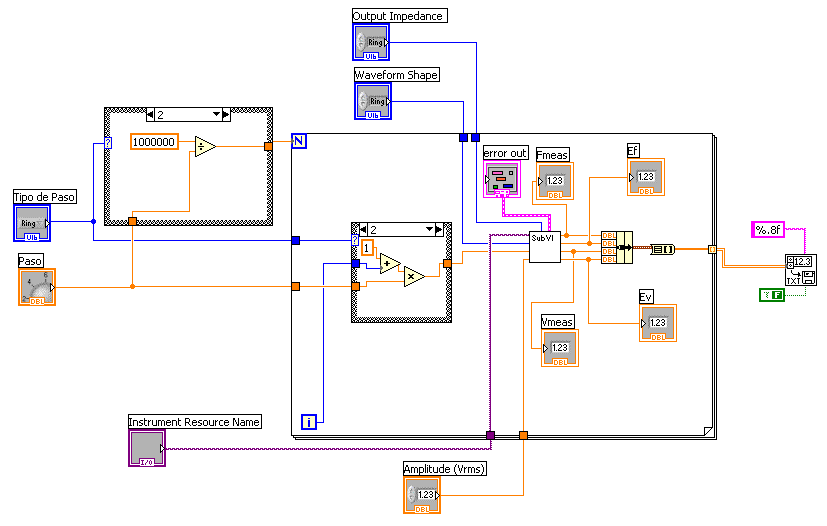
\includegraphics[width=0.8\textwidth]{bloques}}
 \vspace{0.5cm}
 \caption{Instrumento Dise�ado}
 \label{fig:vimejorado}
\end{figure}

El subVI de nombre \emph{subVI}, es el que hemos generado a partir del apartado 1 de la pr�ctica. Sus entradas, de arriba abajo son: 

\begin{itemize}
 \item Impedancia de salida
 \item Instrumento y direcci�n
 \item Forma de onda
 \item Frecuencia (esta ser� la que autom�ticamente vaya ajust�ndose al paso seleccionado durante la ejecuci�n)
 \item Amplitud en Vef.
\end{itemize}

El tipo de barrido de frecuencias se puede seleccionar en el men� \emph{Tipo de Paso}, seg�n se desee (octavas, d�cadas o User Defined). La opci�n de paso definido por el usuario permite ajustar el paso al valor que se desee mediante el dial de la izquieda.

A continuaci�n se muestran las capturas de pantalla de algunos generados por el instrumento con los resultados de las medidas (figura \ref{fig:txtfiles})

\begin{figure}[H]
 \centering
 \subfloat[Paso de Octavas]{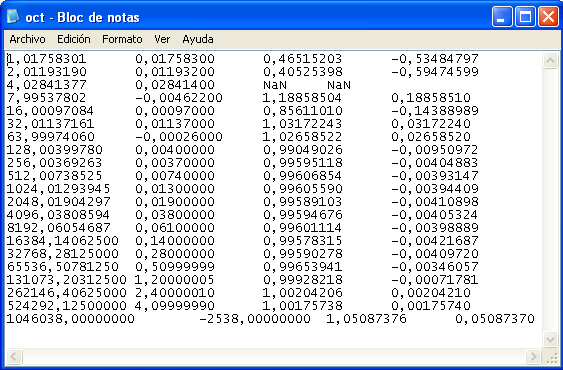
\includegraphics[width=0.6\textwidth]{txtOct}}
 \vspace{0.5cm}
 \subfloat[Paso de D�cadas]{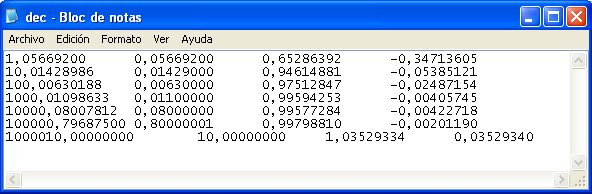
\includegraphics[width=0.6\textwidth]{txtDec}}
 \vspace{0.5cm}
 \subfloat[Paso de 100kHz definido por el usuario]{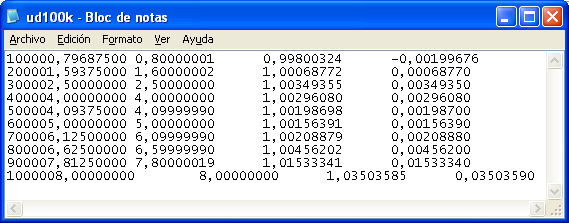
\includegraphics[width=0.6\textwidth]{txtUD100k}}
 \vspace{0.5cm}
 \caption{Capturas de pantalla de los ficheros generados}
 \label{fig:txtfiles}
\end{figure}

\end{document}